\documentclass[11pt,a4paper]{article}
\usepackage[utf8]{inputenc}
\usepackage[vietnamese]{babel}
\usepackage{amsmath,amssymb}
\usepackage[version=4]{mhchem}
\usepackage{geometry}
\geometry{top=0.65cm,bottom=0.65cm,left=1.25cm,right=1.25cm,headheight=20pt,headsep=3pt,footskip=9pt}
\usepackage{graphicx}
\usepackage{xcolor}
\usepackage{tabularx}
\usepackage{array}
\usepackage{tikz}
\usepackage{multicol}
\usepackage{fancyhdr}
\usepackage{enumitem}

\definecolor{hfRed}{HTML}{D32F2F}
\definecolor{hfGreen}{HTML}{8BC390}
\definecolor{mainGreen}{HTML}{2E7D32}

\usepackage{ex_test}

\pagestyle{fancy}
\fancyhf{}
\renewcommand{\headrulewidth}{0.75pt}
\renewcommand{\headrule}{\hbox to\headwidth{\color{hfGreen}\leaders\hrule height \headrulewidth\hfill}}
\renewcommand{\footrulewidth}{0.75pt}
\renewcommand{\footrule}{\hbox to\headwidth{\color{hfGreen}\leaders\hrule height \footrulewidth\hfill}}

\fancyhead[L]{\small\itshape\color{hfRed}Tài liệu lưu hành nội bộ}
\fancyhead[R]{\small\color{hfRed}Thầy \textbf{TRẦN VĂN THẠNH} - 0777.470.803}

\fancyfoot[L]{\footnotesize\itshape\color{hfRed}CS1: 6/15 Nguyễn Hoàng, P. Kim Long, TP Huế \quad|\quad CS2: 24 Đặng Thái Thân, TP Huế}
\fancyfoot[R]{\small\textbf{\color{hfRed}Trang \thepage}}

\setlength{\parindent}{0pt}
\setlength{\parskip}{0.0pt}

\def\loigiai#1{}

\begin{document}
\Opensolutionfile{ans}[ans-de21-hs]

\noindent
\begin{minipage}[t]{0.48\textwidth}
	\textbf{SỞ GIÁO DỤC VÀ ĐÀO TẠO THỪA THIÊN HUẾ}\\
	\textbf{TRƯỜNG THPT HAI BÀ TRƯNG}\\
	\textbf{ĐỀ CHÍNH THỨC}\\
	\textit{(Đề thi có 04 trang)}
\end{minipage}\hfill
\begin{minipage}[t]{0.48\textwidth}
	\raggedleft
	\textbf{\color{mainGreen}ĐỀ KIỂM TRA ĐỊNH KỲ CHƯƠNG 7 (KIM LOẠI NHÓM IA \& IIA)}\\
	\textbf{MÔN: HOÁ HỌC -- LỚP 12}\\
	\textit{Thời gian làm bài: 50 phút (không kể thời gian phát đề)}\\
	\textbf{Mã đề thi: 121}
\end{minipage}


\vspace{1pt}
\noindent\textit{Họ, tên thí sinh: \dots\dots\dots\dots\dots\dots\dots\dots\dots\dots\dots\dots\dots\dots\dots\dots\dots\dots\dots\dots\dots\dots Lớp: \dots\dots\dots\dots SBD: \dots\dots\dots\dots}\\
\noindent\textit{(Cho biết nguyên tử khối: H = 1; C = 12; N = 14; O = 16; Na = 23; Mg = 24; Al = 27; P = 31; S = 32; Cl = 35,5; K = 39; Ca = 40; Fe = 56; Cu = 64; Zn = 65; Br = 80; Rb = 85,5; Ag = 108; Cs = 133; Ba = 137).}

\vspace{1pt}
\noindent
\textbf{PHẦN I (4,5 điểm -- 18 câu): Câu trắc nghiệm nhiều phương án lựa chọn.}\\
\textit{Thí sinh trả lời từ câu 1 đến câu 18. Mỗi câu hỏi thí sinh chỉ chọn một phương án.}

\begin{ex}
Chất nào sau đây tác dụng được với dung dịch \ce{KHCO3}?
\choice
{\ce{K2SO4}.}
{\ce{KNO3}.}
{\ce{HCl}.}
{\ce{KCl}.}
\loigiai{}
\end{ex}

\begin{ex}
Dung dịch \ce{Na2CO3} tác dụng được với dung dịch nào sau đây?
\choice
{\ce{Na2SO4}.}
{\ce{KNO3}.}
{\ce{KOH}.}
{\ce{CaCl2}.}
\loigiai{}
\end{ex}

\begin{ex}
Dung dịch nào sau đây phản ứng với dung dịch \ce{HCl} dư tạo ra chất khí?
\choice
{\ce{Ba(OH)2}.}
{\ce{Na2CO3}.}
{\ce{K2SO4}.}
{\ce{Ca(NO3)2}.}
\loigiai{}
\end{ex}

\begin{ex}
Trong cốc nước chứa 0,01 mol \ce{Na+}; 0,02 mol \ce{Ca^2+}; 0,01 mol \ce{Mg^2+}; 0,05 mol \ce{HCO3-} và 0,02 mol \ce{Cl-}. Đun sôi cốc nước hồi lâu, nước thu được là
\choice
{Nước cứng tạm thời.}
{Nước cứng vĩnh cửu.}
{Nước mềm.}
{Nước cứng toàn phần.}
\loigiai{}
\end{ex}

\begin{ex}
Phản ứng giải thích sự hình thành thạch nhũ trong các hang động núi đá vôi là:
\choice
{$\ce{CaCO3 + CO2 + H2O -> Ca(HCO3)2}$.}
{$\ce{CaCO3 + 2HCl -> CaCl2 + CO2 + H2O}$.}
{$\ce{CaCO3 ->[t^\circ] CaO + CO2}$.}
{$\ce{Ca(HCO3)2 <=> CaCO3 + CO2 + H2O}$.}
\loigiai{}
\end{ex}

\begin{ex}
Nước thải công nghiệp thường chứa các ion kim loại nặng như \ce{Hg^2+}, \ce{Pb^2+}, \ce{Fe^3+}. Để xử lí triệt để và làm giảm nồng độ của các ion kim loại nặng với chi phí thấp nhất, người ta sử dụng dung dịch chất nào sau đây?
\choice
{\ce{HCl}.}
{\ce{NaCl}.}
{\ce{Ca(OH)2}.}
{\ce{K2SO4}.}
\loigiai{}
\end{ex}

\begin{ex}
Cho các dãy kim loại sau: Fe, Na, K, Cu và Li. Số kim loại trong dãy tác dụng được với nước ở nhiệt độ thường là
\choice
{1.}
{2.}
{3.}
{4.}
\loigiai{}
\end{ex}

\begin{ex}
Nguyên tắc cơ bản để làm mềm nước cứng là làm giảm nồng độ của
\choice
{ion \ce{Ca^2+}, \ce{Mg^2+}.}
{ion \ce{HCO3-}.}
{ion \ce{OH-}, \ce{SO4^2-}.}
{ion \ce{Ca^2+}.}
\loigiai{}
\end{ex}

\begin{ex}
Kim loại nhóm IIA có nhiệt độ nóng chảy, nhiệt độ sôi, khối lượng riêng biến đổi không theo quy luật như kim loại kiềm nhóm IA, nguyên nhân chủ yếu là do các kim loại nhóm IIA có
\choice
{điện tích hạt nhân khác nhau.}
{cấu hình electron khác nhau.}
{bán kính nguyên tử khác nhau.}
{kiểu mạng tinh thể khác nhau.}
\loigiai{}
\end{ex}

\newpage

\begin{ex}
Khi để vôi sống trong không khí ẩm một thời gian sẽ có hiện tượng một phần bị chuyển hoá trở lại thành đá vôi. Khí nào sau đây có trong không khí gây ra hiện tượng trên?
\choice
{Oxygen.}
{Methane.}
{Nitrogen.}
{Carbon dioxide.}
\loigiai{}
\end{ex}

\begin{ex}
Đun nóng tinh thể \ce{CaF2} với dung dịch \ce{H2SO4} đặc ở nhiệt độ khoảng $250^\circ\text{C}$, thu được khí nào sau đây?
\choice
{\ce{SO2}.}
{\ce{F2}.}
{\ce{HF}.}
{\ce{H2S}.}
\loigiai{}
\end{ex}

\begin{ex}
Cho dung dịch \ce{HCl} vào dung dịch X thấy có hiện tượng sủi bọt khí; nếu cho dung dịch \ce{Ca(OH)2} vào dung dịch X thì sinh ra kết tủa trắng. Dung dịch X là
\choice
{\ce{Na2SO4}.}
{\ce{KNO3}.}
{\ce{Ca(HCO3)2}.}
{\ce{BaCl2}.}
\loigiai{}
\end{ex}

\begin{ex}
Cho một mẩu Na vào dung dịch \ce{MgSO4} dư, thu được kết tủa X và chất khí Y. Hai chất X, Y lần lượt là
\choice
{Mg và \ce{H2}.}
{\ce{Mg(OH)2} và \ce{H2}.}
{Mg và \ce{O2}.}
{\ce{Na2SO4} và \ce{H2}.}
\loigiai{}
\end{ex}

\begin{ex}
Trong cốc nước chứa nhiều các ion sau: \ce{Ca^2+}, \ce{Mg^2+}, \ce{Cl-}, \ce{SO4^2-}. Nước trong cốc trên thuộc loại
\choice
{có tính cứng vĩnh cửu.}
{không có tính cứng.}
{có tính cứng tạm thời.}
{có tính cứng toàn phần.}
\loigiai{}
\end{ex}

\begin{ex}
Nhận định nào \textbf{không} đúng về cấu tạo và tính chất của các kim loại nhóm IIA?
\choice
{Khối lượng riêng tương đối nhỏ, là những kim loại nhẹ hơn nhôm (trừ Ba).}
{Độ cứng cao hơn kim loại nhóm IA, nhưng mềm hơn kim loại nhôm.}
{Mạng tinh thể của chúng đều có kiểu lập phương tâm khối.}
{Nhiệt độ nóng chảy và nhiệt độ sôi tương đối thấp (trừ Be).}
\loigiai{}
\end{ex}

\begin{ex}
Cho các nhận định sau về tác hại của nước cứng:\\
(1) Làm giảm bọt và giảm khả năng tẩy rửa khi giặt quần áo bằng xà phòng.\\
(2) Làm đường ống dẫn nước bị đóng cặn, giảm lưu lượng dòng chảy.\\
(3) Làm thức ăn lâu chín và giảm mùi vị đặc trưng khi nấu nướng.\\
(4) Làm nồi hơi bị phủ cặn cách nhiệt, gây tốn nhiên liệu và có nguy cơ gây nổ lò hơi.\\
Số nhận định đúng là
\choice
{1.}
{2.}
{3.}
{4.}
\loigiai{}
\end{ex}

\begin{ex}
Phát biểu nào sau đây \textbf{không} đúng?
\choice
{Đun sôi nước cứng chỉ làm mềm nước cứng tạm thời.}
{Dung dịch \ce{Na2CO3} làm mềm nước cứng tạm thời, nước cứng vĩnh cửu.}
{Dung dịch \ce{NH4Cl} làm mềm nước cứng.}
{Cho dung dịch \ce{Ca(OH)2} vừa đủ làm mềm nước cứng tạm thời.}
\loigiai{}
\end{ex}

\begin{ex}
Cho sơ đồ chuyển hoá hoá học sau:
\par\vspace{1pt}\centerline{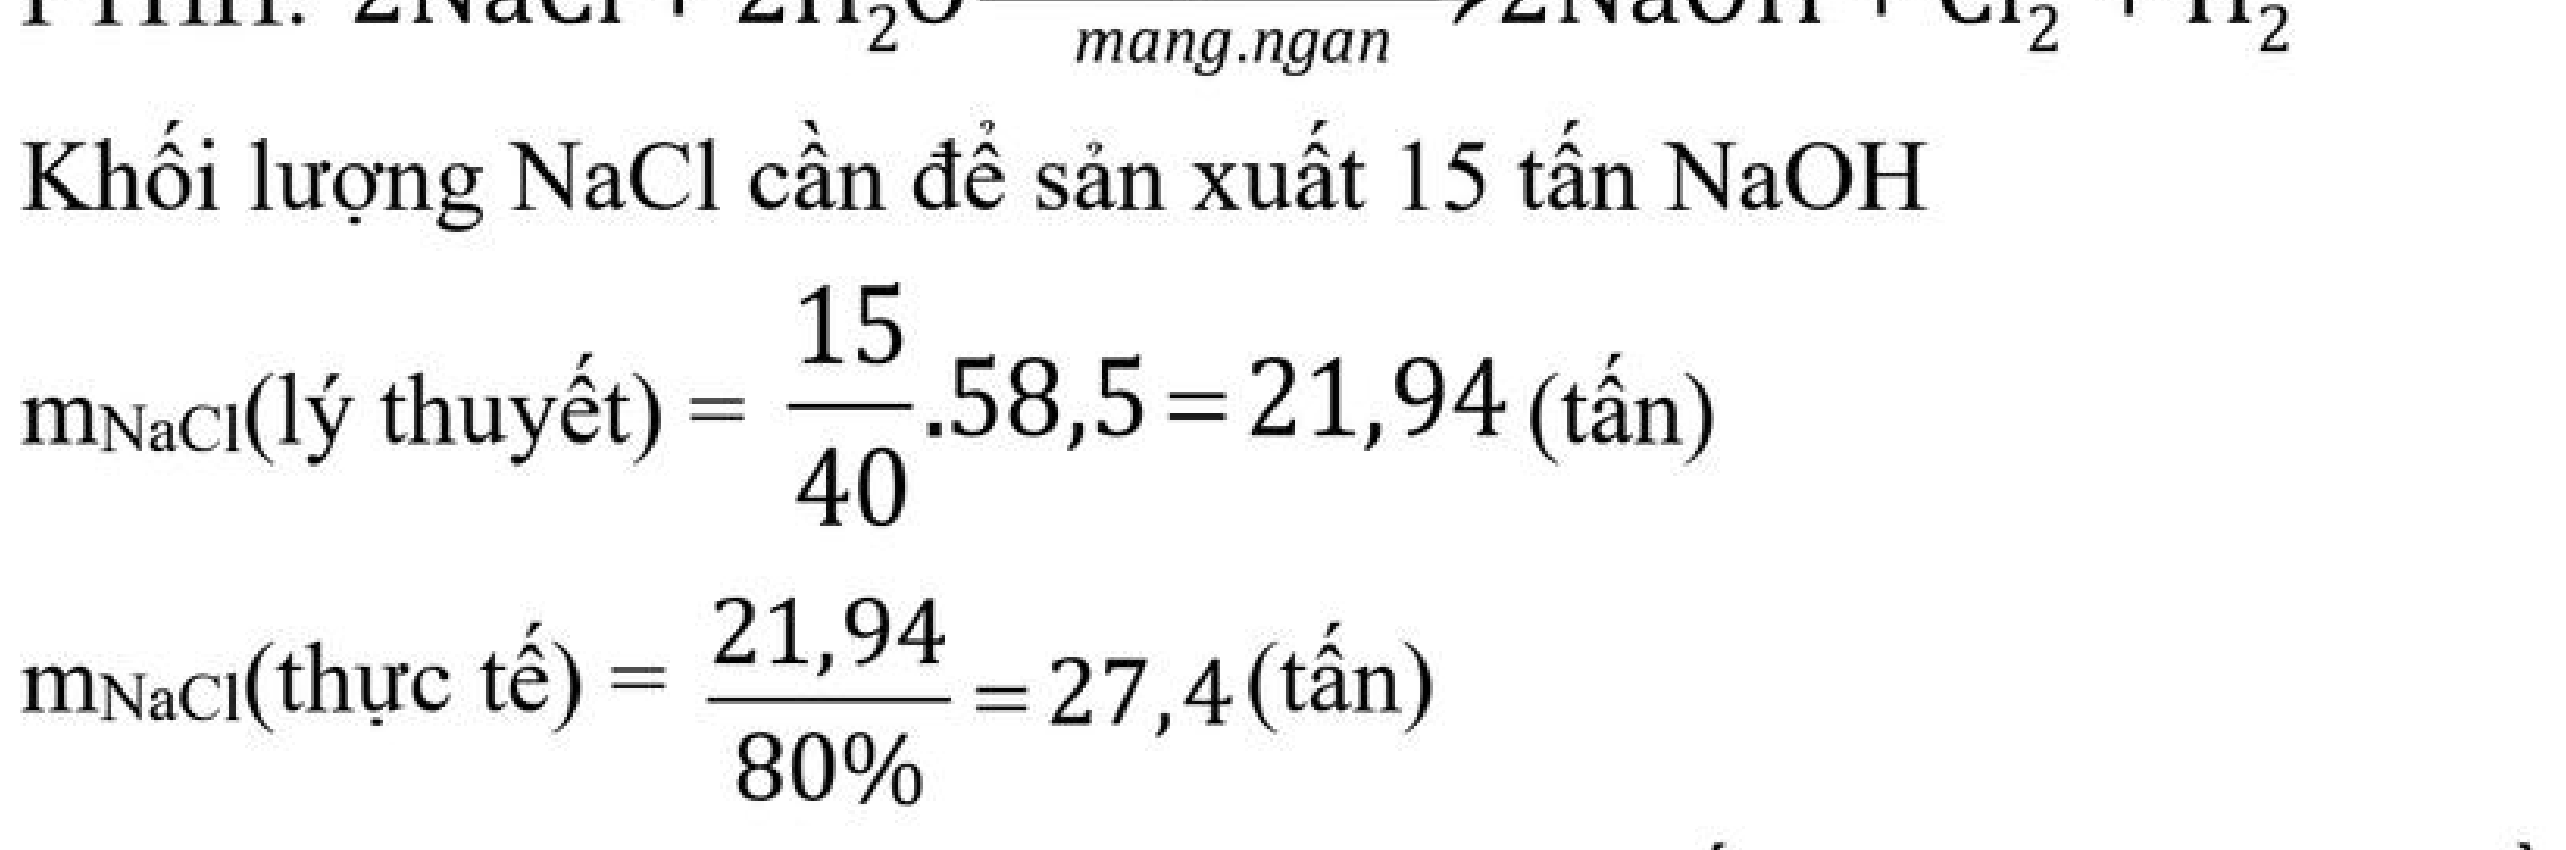
\includegraphics[height=1.45cm]{images_crop_de21/p1_cau18_so_do.png}}\vspace{1pt}
Chất X trong sơ đồ trên có thể là
\choice
{\ce{BaCO3}.}
{\ce{CaCO3}.}
{\ce{BaSO3}.}
{\ce{MgCO3}.}
\loigiai{}
\end{ex}

\newpage

\noindent
\textbf{PHẦN II (4,0 điểm -- 4 câu): Câu trắc nghiệm đúng sai.}\\
\textit{Thí sinh trả lời từ câu 1 đến câu 4. Trong mỗi ý a), b), c), d) ở mỗi câu, thí sinh chọn đúng hoặc sai.}

\setcounter{ex}{0}

\begin{ex}
Trong tự nhiên, các nguyên tố nhóm IA chỉ tồn tại ở dạng hợp chất (chủ yếu là dạng muối). Sodium và potassium là hai nguyên tố phổ biến trong vỏ Trái Đất, có nhiều trong nước biển, muối mỏ, quặng halite (\ce{NaCl}), quặng sylvinite (\ce{NaCl.KCl}).
\choiceTF
{Trong đời sống hàng ngày, sodium chloride được dùng làm gia vị, bảo quản và chế biến thực phẩm.}
{Điện phân dung dịch \ce{NaCl} bão hoà có màng ngăn điện cực được ứng dụng trong công nghiệp để sản xuất nước Javel.}
{Trong công nghiệp, khí chlorine được sản xuất bằng cách điện phân dung dịch muối ăn bão hoà có màng ngăn xốp.}
{Sodium carbonate là nguyên liệu quan trọng để sản xuất thuỷ tinh, xà phòng, bột giặt, giấy, sợi và chất tẩy rửa.}
\loigiai{}
\end{ex}

\begin{ex}
Khi nồng độ acid trong dịch vị dạ dày tăng cao có thể gây ra viêm loét dạ dày, tá tràng. Để giảm bớt nồng độ acid trong dịch vị dạ dày người ta thường dùng thuốc đau dạ dày có chứa thành phần chính là muối X.
\choiceTF
{Muối X là sodium bicarbonate có công thức hoá học là \ce{Na2CO3}.}
{Muối X còn được dùng để tạo độ xốp cho các loại bánh nướng, làm mềm thực phẩm.}
{Muối X bị phân huỷ khi đun nóng.}
{Trong công nghiệp hoá chất, muối X được sản xuất chủ yếu bằng phương pháp Solvay.}
\loigiai{}
\end{ex}

\begin{ex}
Bảng sau đây cho biết thông số một số tính chất vật lí cơ bản của các kim loại nhóm IIA:
\par\vspace{1pt}\centerline{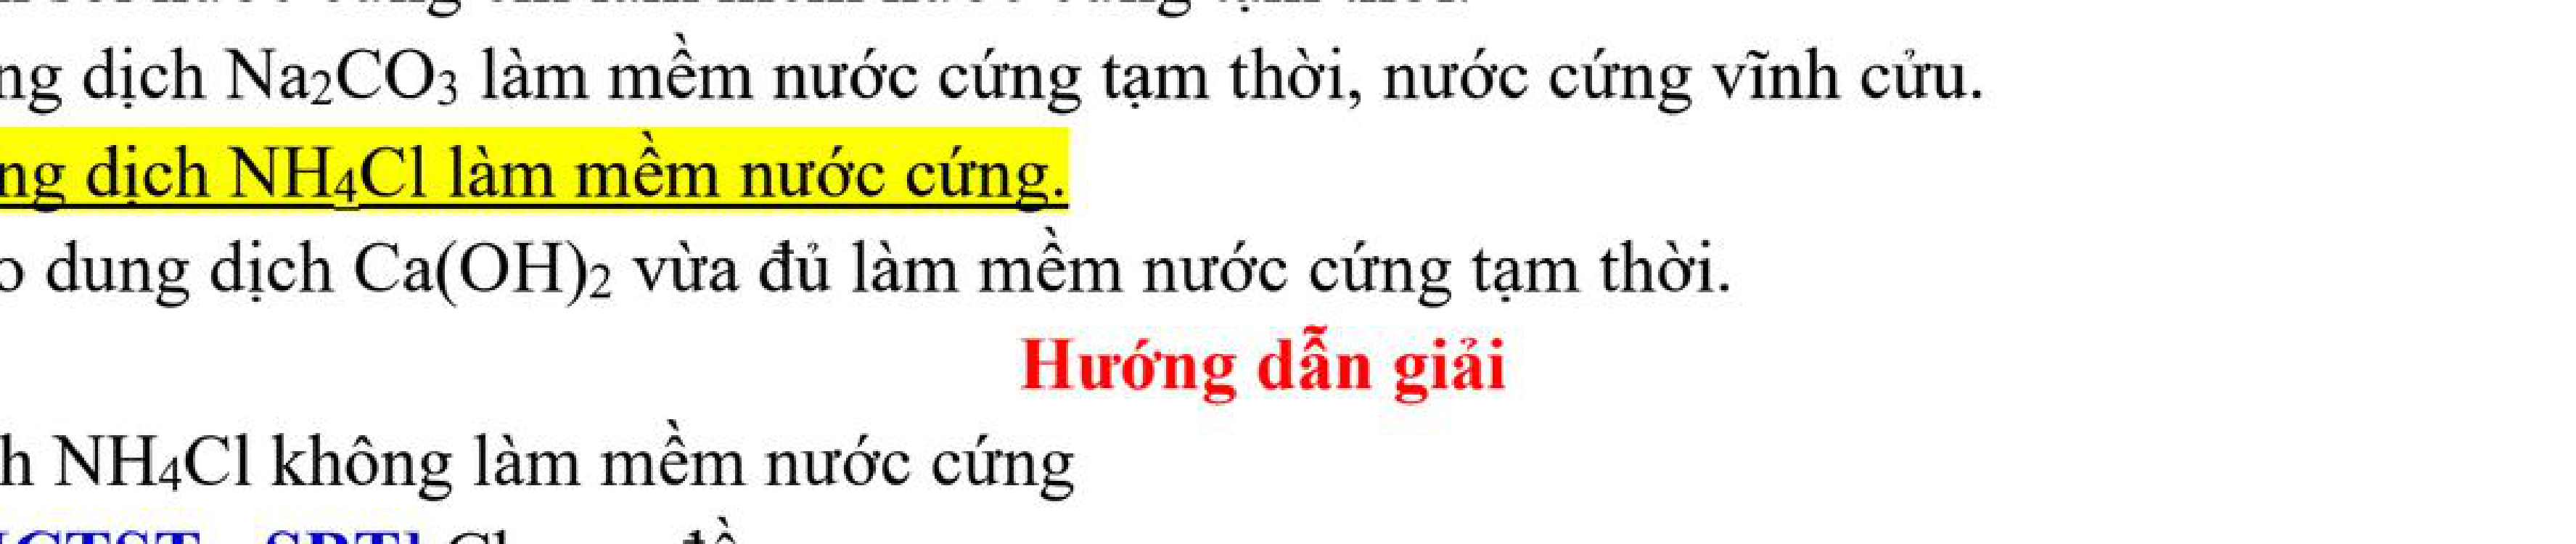
\includegraphics[height=1.5cm]{images_crop_de21/p2_cau3_bang_tinh_chat.png}}\vspace{1pt}
\choiceTF
{Nhiệt độ sôi tăng dần từ Be đến Ba.}
{Khối lượng riêng tăng dần đều đặn từ trên xuống dưới từ Mg đến Ba.}
{Độ cứng của các kim loại tăng dần từ Be đến Ba.}
{Nhiệt độ nóng chảy giảm dần đều đặn từ Be đến Ba.}
\loigiai{}
\end{ex}

\begin{ex}
Cho các phản ứng hoá học xảy ra theo sơ đồ sau:\\
(1) $\ce{2X1 + 2H2O ->[dpdd, co mang ngan] 2X2 + X3 + H2}$\\
(2) $\ce{2X2 + X4 -> BaCO3 v + K2CO3 + 2H2O}$\\
(3) $\ce{X4 + X5 ->[1:1] BaSO4 v + 2CO2 ^ + 2H2O}$
\choiceTF
{Hợp chất $\text{X}_2$ là potassium hydroxide (KOH).}
{Đơn chất $\text{X}_3$ là chất khí có màu vàng lục nhạt.}
{Muối $\text{X}_4$ là muối acid (muối hydrogencarbonate).}
{Khi đun nóng dung dịch muối $\text{X}_4$ thì thu được kết tủa trắng.}
\loigiai{}
\end{ex}

\newpage

\noindent
\textbf{PHẦN III (1,5 điểm -- 6 câu): Câu trắc nghiệm yêu cầu trả lời ngắn.}\\
\textit{Thí sinh trả lời từ câu 1 đến câu 6.}

\setcounter{ex}{0}

\begin{ex}
Trong công nghiệp, quá trình sản xuất soda bằng phương pháp Solvay đi từ các nguyên liệu ban đầu là muối ăn (\ce{NaCl}), đá vôi (\ce{CaCO3}) và ammonia (\ce{NH3}). Có bao nhiêu phương trình hoá học chủ yếu đã xảy ra trong toàn bộ quy trình trên?
\par\noindent\textit{Trả lời:} \dotfill
\loigiai{}
\end{ex}

\begin{ex}
Cho các nguyên tố sau: Kr, Ca, Sr, Li, Ni, Rb. Có bao nhiêu nguyên tố là kim loại kiềm (nhóm IA) trong dãy trên?
\par\noindent\textit{Trả lời:} \dotfill
\loigiai{}
\end{ex}

\begin{ex}
Cho các chất sau: \ce{Ca(OH)2}, \ce{Na2CO3}, \ce{Na3PO4}, \ce{NaOH}, \ce{KCl}. Có bao nhiêu chất có thể dùng để làm mềm nước có tính cứng vĩnh cửu?
\par\noindent\textit{Trả lời:} \dotfill
\loigiai{}
\end{ex}

\begin{ex}
Cho dung dịch của 4 chất sau đều trong suốt và không màu: \ce{NaCl}, \ce{Na2SO4}, \ce{KCl}, \ce{LiNO3}. Chỉ dùng ngọn lửa không màu của đèn khí thì có thể nhận biết được bao nhiêu dung dịch riêng biệt trong số 4 dung dịch trên?
\par\noindent\textit{Trả lời:} \dotfill
\loigiai{}
\end{ex}

\begin{ex}
Ở $20^\circ\text{C}$, độ tan của \ce{NaCl} trong nước là 35,9 gam trong 100 gam nước. Ở nhiệt độ này, dung dịch \ce{NaCl} bão hoà có nồng độ phần trăm là $a\%$. Xác định giá trị của $a$ (làm tròn kết quả đến hàng phần mười).
\par\noindent\textit{Trả lời:} \dotfill
\loigiai{}
\end{ex}

\begin{ex}
Một loại thuốc kháng acid dạ dày có tên thương mại là Rolaids chứa thành phần hoạt chất chính là dihydroxyaluminum sodium carbonate có công thức \ce{NaAl(OH)2CO3}. Mỗi viên thuốc chứa 0,334 gam hoạt chất \ce{NaAl(OH)2CO3}. Một cốc nước giải khát có thể tích 250 mL và có $\text{pH} = 3{,}0$. Giả thiết phản ứng trung hòa xảy ra hoàn toàn theo phương trình: $\ce{NaAl(OH)2CO3 + 4H+ -> Na+ + Al^3+ + CO2 + 3H2O}$. Tính số viên thuốc Rolaids cần dùng để trung hòa hết lượng acid có trong cốc nước giải khát trên (làm tròn kết quả đến hai chữ số thập phân).
\par\noindent\textit{Trả lời:} \dotfill
\loigiai{}
\end{ex}

\Closesolutionfile{ans}
\end{document}
